\documentclass[conference,compsoc]{IEEEtran}

% *** CITATION PACKAGES ***
%
\ifCLASSOPTIONcompsoc
  % IEEE Computer Society needs nocompress option
  % requires cite.sty v4.0 or later (November 2003)
  \usepackage[nocompress]{cite}
\else
  % normal IEEE
  \usepackage{cite}
\fi

% *** GRAPHICS RELATED PACKAGES ***
%
\ifCLASSINFOpdf
\else
\fi

% correct bad hyphenation here
\hyphenation{op-tical net-works semi-conduc-tor}
\usepackage{amssymb} %mathematical packages to write correct' formulas
\usepackage{amsmath}
\usepackage{graphicx}
\usepackage{float}
\usepackage{wrapfig} 
\usepackage{dblfloatfix}
\usepackage[table,xcdraw]{xcolor} 
\begin{document}
\setlength{\parindent}{15pt}


\title{Comparative analysis of dynamic routing protocol in data center}


% author names and affiliations
% use a multiple column layout for up to three different
% affiliations
\author{
\IEEEauthorblockN{Lukasz Joksch}
\IEEEauthorblockA{Department of Electronics,\\Wroclaw University of Science and Technology\\Wroclaw, Poland\\
E-mail: 200963@student.pwr.edu.pl}
\and
\IEEEauthorblockN{Tomasz Kowalik}
\IEEEauthorblockA{Department of Electronics,\\Wroclaw University of Science and Technology\\Wroclaw, Poland\\
E-mail: 200943@student.pwr.edu.pl}

}

% conference papers do not typically use \thanks and this command
% is locked out in conference mode. If really needed, such as for
% the acknowledgment of grants, issue a \IEEEoverridecommandlockouts
% after \documentclass

% for over three affiliations, or if they all won't fit within the width
% of the page (and note that there is less available width in this regard for
% compsoc conferences compared to traditional conferences), use this
% alternative format:
% 
%\author{\IEEEauthorblockN{Michael Shell\IEEEauthorrefmark{1},
%Homer Simpson\IEEEauthorrefmark{2},
%James Kirk\IEEEauthorrefmark{3}, 
%Montgomery Scott\IEEEauthorrefmark{3} and
%Eldon Tyrell\IEEEauthorrefmark{4}}
%\IEEEauthorblockA{\IEEEauthorrefmark{1}School of Electrical and Computer Engineering\\
%Georgia Institute of Technology,
%Atlanta, Georgia 30332--0250\\ Email: see http://www.michaelshell.org/contact.html}
%\IEEEauthorblockA{\IEEEauthorrefmark{2}Twentieth Century Fox, Springfield, USA\\
%Email: homer@thesimpsons.com}
%\IEEEauthorblockA{\IEEEauthorrefmark{3}Starfleet Academy, San Francisco, California 96678-2391\\
%Telephone: (800) 555--1212, Fax: (888) 555--1212}
%\IEEEauthorblockA{\IEEEauthorrefmark{4}Tyrell Inc., 123 Replicant Street, Los Angeles, California 90210--4321}}




% use for special paper notices
%\IEEEspecialpapernotice{(Invited Paper)}




% make the title area
\maketitle

% As a general rule, do not put math, special symbols or citations
% in the abstract
\begin{abstract}
During the last few decades all kind of computer networks has rapidly grown. It is noticeable espacially in big companies, which have their own data centres. They require  special solutions, diffrent in diffrent data centres. This solutions have to cope the most difficult requirements. It is very important to choose wisely diffrent kinds of mechanism used in networks in example proper dynamic routing protocol. It is hard to say which one will be optimal in diffrent cases. In this paper, we will investigate which popular dynamic routing protocol is the best in given cases. We also compare them with latest trend in networks – Software-Defined Networking.
\end{abstract}


\textbf{\\ Keywords - Dynamic routing protocols, EIGRP, OSPF, IS-IS, RIP, SDN}

\section{Introduction}

Computer networks is one of the fastest growing area of technology in these days. At the beginning, they were used usually to communicate between people or to share a files. Nowadays modern networks brings much more functions: printer sharing, video conferencing, streaming video and music, entertainment and more. Large data centers use lots of applications and technologies which make work easier and more efficient. Therefore modern network must be fast and efficient too.
\\ \indent In past networks were different. For example it was necessary to have equipment made by the same vendor. Otherwise computers, printers or something else cannot communicate with each other. This problem was solved introducing the Open Systems Interconnection (OSI) reference model by the International Organization for Standardization (ISO). The OSI model was meant to help vendors create interoperable network devices and software in the form of protocols so that networks from different vendors could work with each other.
\\ \indent Actually, the most popular network layer protocol for connecting computer networks is Internet Protocol (IP). Network layer is responsible mostly for finding the best way from one host from one subnet to another host in another subnet. It is very difficult, especially in large networks. However, there are dynamic routing protocols, which do it automatically. Nowadays, the most widely used intra domain routing protocols are Open Shortest Path First (OSPF) [23], Enhanced Interior Gateway Routing Protocol (EIGRP) [22], Intermediate System to Intermediate System (IS-IS) [23] and Routing Information Protocol (RIP) [21]. Lately, Software-Defined Networking were introduced. It is new solution for networks and it is said it will be future of networking. It is new kind of technology.
\\ \indent This article shows real time and simulation comparative between dynamic routing protocols such as OSPF, EIGRP, IS-IS, RIP and new solution – Software-Defined Networking (SDN) [16-20, 25]. Realistic survey were made using Cisco routers and the simulations were carried out by using the GNS3 simulator.


\section{Related works}

Works [1-5 and 7-11] testing the routing protocols using different simulators, like: OPNET, GNS3, NT-3 and Cisco Packet Tracer. In their studies, authors of works [1-5 and 7-11], create various scenarios to compare performance of protocols such as EIGRP, OSPF, RIP, IS-IS. They usually survey convergence duration, traffic sent, link utilization, throughput and bandwidth. E. Shewandagn Lemma, S. A. Hussain, W. W. Anjelo, S. Farhangi, A. Rostami, S. Golmohammadi, as in [1-2], also were testing combination of various dynamic routing protocols. Articles [16-20] present solutions used in Software-Defined Networking. Authors shows their own algorithms, combinations of existing technology or compare existing technology with well-known dynamic routing protocols such as OSPF.

\section{Dynamic routing protocols}
\begin{itemize}
\item 
\emph{General information}\\\\
In IP networks, the main task of a routing protocol is to carry packets forwarded from one node to another. In a network, routing can be defined as transmitting information from a source to a destination by hopping one-hop or multi hop. Routing protocols should provide at least two facilities: selecting routes for different pairs of source/destination nodes and, successfully transmitting data to a given destination.
\\ The main objective of routing protocols is to determine the best path from a source to a destination. A routing algorithm uses different metrics based on a single or on several properties of the path in order to determine the best way to reach a given network. Conventional routing protocols used in interior gateway networks are classified as Link State Routing Protocols and Distance Vector Routing Protocols.\\

\item
\emph{Routing Information Protocol}\\\\
Distance vector routing algorithm assumes that each router maintains a table (e.g., a vector) that preserves the best known distance to each destination and the line to be followed to get there.
\\ A distance vector protocol maintains and transmits tables routing in which are listed all known networks and the distances to each of them.
\\ Distance vector routing algorithm is also known by other names such as distributed routing algorithm Bellman-Ford or Ford-Fulkerson algorithm; named researchers have proposed (Bellman, 1957 Ford and Fulkerson, 1962). When a router to update its routing table, it sends all the essential information from adjacent routers routing table. When it receives a distance vector, checks for changes from the previous distance vector received from the same neighboring router, in which case the result is positive, it will restore the routing table, packets transmitting distance vectors to neighboring routers.
\\ This protocol sends broadcast its routing table every 30 seconds. A packet can contain up to 25 destinations, and the unit measure uses hop count (number of jumps), maximum is 15 routers.\\

\item 
\emph{Open Shortest Path First}\\\\
Link state routing protocols do not change each routing tables, the information provided refers to the state of routers directly connected networks. Routing based on state bonds is widely used in current networks, protocol OSPF (Open Shortest Path First) is used increasingly over the Internet, using an algorithm based on state bonds. Each router discovers that its direct neighbors and communicate this information to other routers, using special packages carrying state links (link state packet). These packets are transmitted by the selective flooding and taken to destination routers update their own data base, the synchronization being performed at intervals of 30 minutes, the LSP packets. Each router maintains a database on which the graph of the network will develop its own routing table. Routers running this protocol accumulates information linkages on the state calculates the shortest path to a given network algorithm is known as Dijsktra algorithm. Each node is labeled with the distance from the source node to it, the over the best way known initially not knowing is no way, all nodes will be labeled with infinity. Initially, all tags are temporary, but when it is discovered that a label is the shortest possible path from the source to that node, it changes its status to become permanent.\\

\item 
\emph{Enhanced Interior Gateway Routing Protocol}\\\\
EIGRP, considered a hybrid routing protocol, is a class of protocols of "distance vector" and was issued in 1992, was an improvement protocol IGRP, both Cisco proprietary and can only operate on Cisco routers. EIGRP can learn in a dynamic way on the routers directly connected to a network, this is similar to the protocol "Hello" used to discover OSPF neighbors on a network. A network equipment EIGRP packets change "hello" to ensure that each neighbor is operational. As in the case of OSPF, the frequency of the exchange of packets based on the type of network where high bandwidth links exchange is carried out at intervals of 5 seconds, and in the case of connections requiring low bandwidth, the packets are exchanged every 60 seconds. EIGRP does not rely on periodic updates to converge in the topology, instead building a table that will contain announcements on neighbors about changes in topology; data is not removed as in distance vector protocols. Topology table information is processed to determine the best path to each destination network, EIGRP implementing an algorithm known as the diffusion update algorithm (DUAL).\\

\item 
\emph{Intermediate System to Intermediate System}\\\\
IS-IS is designed to provide intra domain routing or routing within an area. IS-IS network includes end systems, intermediate system, areas and domains. In IS-IS network, routers are intermediate systems organized into local groups known as areas. Several area are grouped together to form domains. User devices are End systems. 
\\ IS-IS and OSPF are link state routing protocols that can be used for larger networks. IS-IS uses Dijkstra algorithm to determine the shortest path and utilizes a link state database to route packets between intermediate systems. IS-IS usually use two level hierarchical routing in which a level 1 router can identify the topology in the area including every router and host. However, a level 1 router cannot know the identity of routers outside their area. Level 1 routers of are similar to OSPF intra area routers since it has no connections outside. Level 2 routers are not required to identify the topology within level 1 area but there is a possibility that a level 2 router can be a level 1 router in a single area. 
\\ Level 2 of IS-IS is similar to OSPF Area 0 that comprises the backbone Area in order to connect different areas.
\\

\end{itemize}

\section{RESEARCH}
Our research was divided into few steps. First of all we have to made two topologies. Because we made research that could be implement in data center we had to prepare topologies that ensure redundancy, as links as well nodes. 
\\ \indent One of them – smaller – to test on real physical hardware. In this case we use 15 Cisco 2801 routers. All this routers have 2 Fast Ethernet ports and 2 Serial ports. We use all of this ports to connect devices with each other.

\begin{figure}[!h]
  \begin{center}
    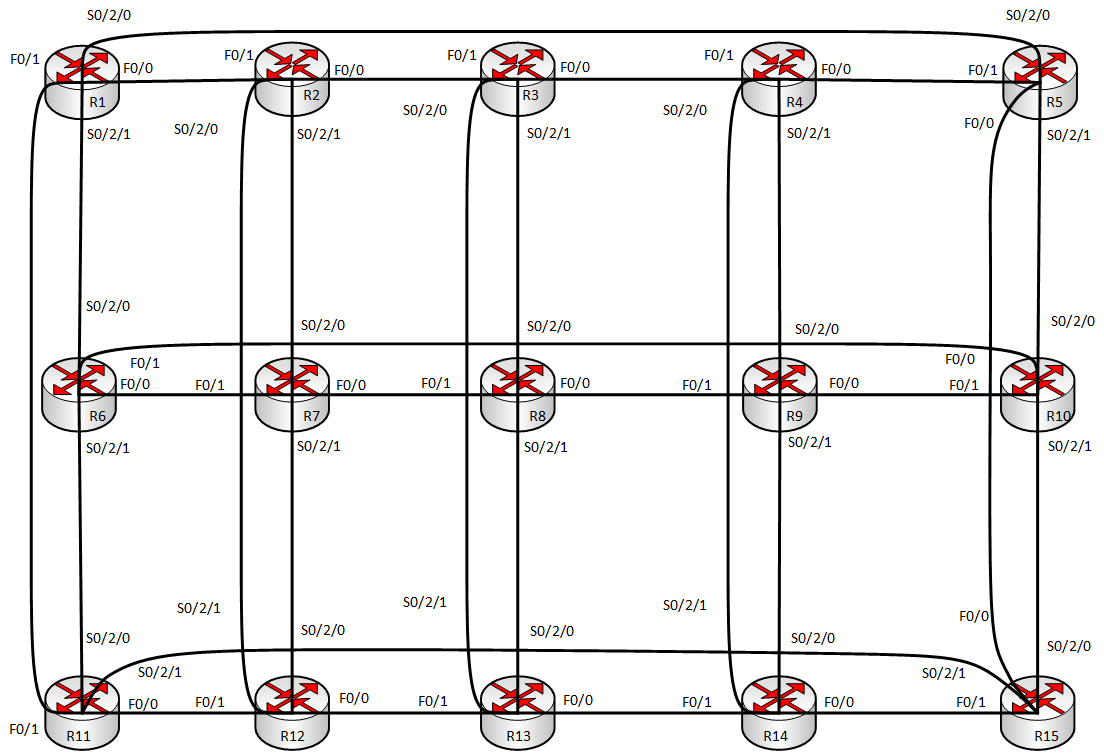
\includegraphics[width=\columnwidth]{images/f1}
  \end{center}
  \caption{Smaller topology with Cisco 2801 routers}
\end{figure}

Second topology – bigger one – was made to do research in GNS3 – network simulator/emulator. This time we were using 30 Cisco 7200 routers with IOS 15. This equipment contains only Fast Ethernet ports. We use 4 of this ports, as in the previous case.


\begin{figure}[!h]
  \centering
  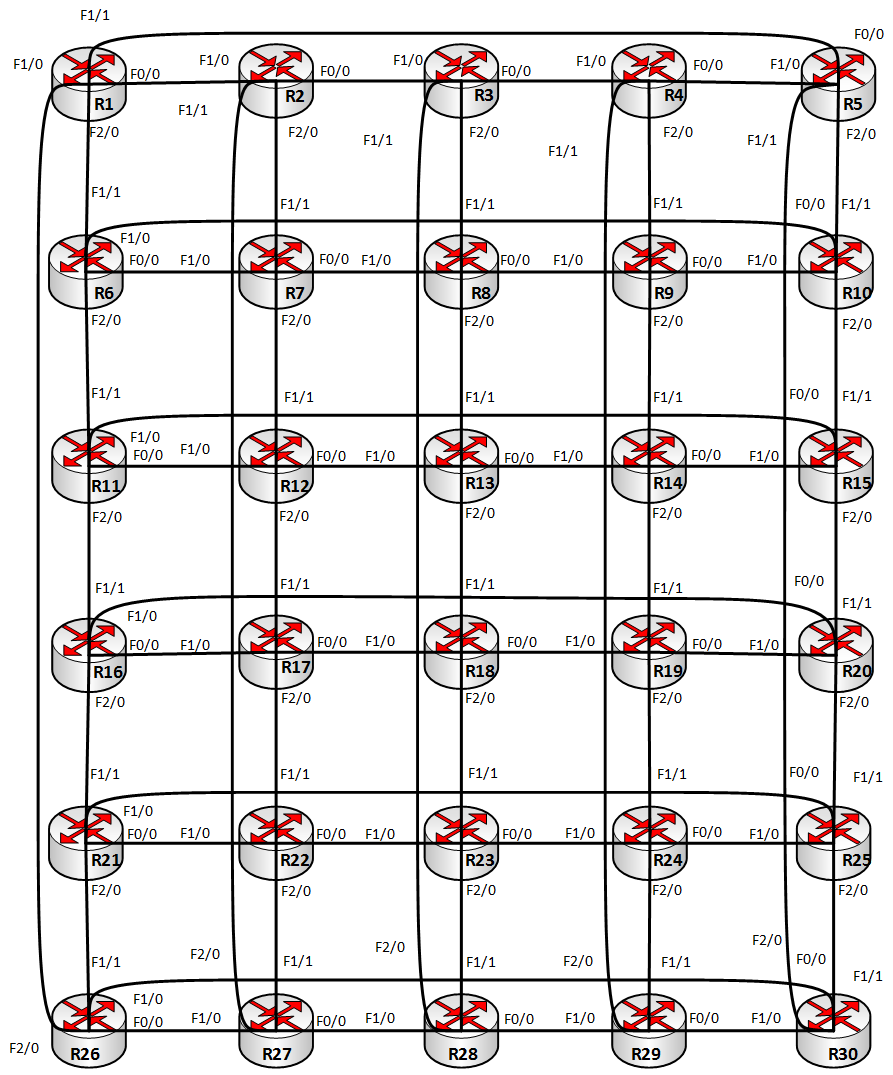
\includegraphics[width=\columnwidth]{images/f2}
  \caption{Bigger topology with Cisco 7200 routers}
\end{figure}



We also prepared configurations for each router separately. Configurations were different in each topology because for example we were using different types of routers or ports. For each topology were prepared 4 different configurations – everyone for other protocol – RIP, IS-IS, OSPF and EIGRP.
We also connect PCs to routers. In Figure 1 PC1 was connected to R1 and PC2 to R13. In Figure 2 PC1 was again connected to R1 and PC2, this time was connected to R18.
In our research we also were using Wireshark. It is the world’s foremost and widely-used network protocol analyzer. It lets us to see what’s happening on our networks at a microscopic level and is the de facto standard across many commercial and non-profit enterprises, government agencies, and educational institutions.
Then we started to ping PC2 from PC1. Then we simulated failure of single link 10 times and also 10 times we simulate failure of single node. This crash test was made for each dynamic routing protocols and for two topologies. Each time we were measuring times of convergence. Every time we also checked which route protocols choose.

\section{ANALYSIS}

After our research we averaged the results and made 4 comparison:
\begin{itemize}
\item Time of convergence of single link failure for smaller topology;
\item Time of convergence of single node failure for smaller topology;
\item Time of convergence of single link failure for bigger topology;
\item Time of convergence of single node failure for bigger topology;

\end{itemize}

\begin{figure}[!h]
  \centering
  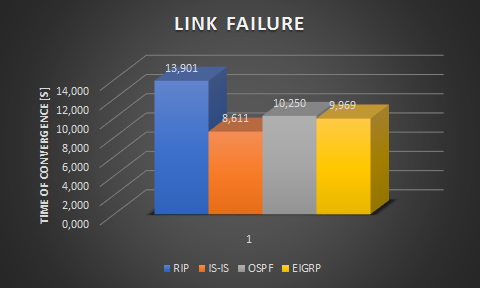
\includegraphics[width=\columnwidth]{images/f3}
  \caption{Time of convergence of single link failure for smaller topology}
\end{figure}

\begin{figure}[!h]
  \centering
  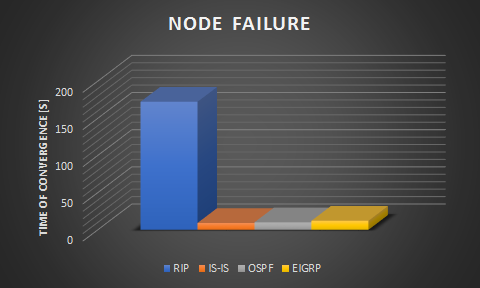
\includegraphics[width=\columnwidth]{images/f4}
  \caption{Time of convergence of single node failure for smaller topology}
\end{figure}


\begin{figure}[!h]
  \centering
  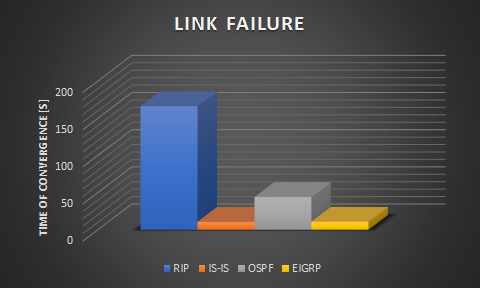
\includegraphics[width=\columnwidth]{images/f5}
  \caption{Time of convergence of single link failure for bigger }
\end{figure}

\begin{figure}[!h]
  \centering
  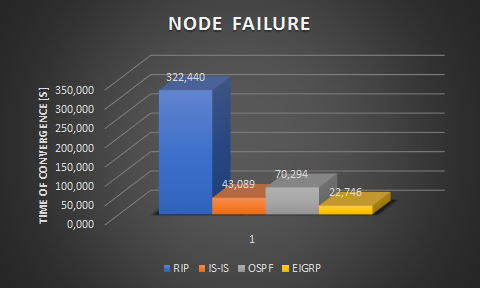
\includegraphics[width=\columnwidth]{images/f6}
  \caption{Time of convergence of single node failure for bigger topology}
\end{figure}






\indent As we can see on Figure 3 for smaller topology the slowest dynamic routing protocol in the case of damage of single link is the RIP. It is more than 1,5 times slower than the fastest routing protocol – IS-IS. More than one second slower than IS-IS protocol is EIGRP.
\\ \indent Figure 4 shows us that, again, the fastest dynamic routing protocol is IS-IS. A bit slower are EIGRP and OSPF. Almost 20 times slower in this juxtaposition is RIP.
\\ \indent For bigger topology we made two another charts (Figure 5 and Figure 6). Time of convergence of single link failure for bigger topology, shows on Figure 5, is the best for IS-IS as well as for smaller topology. Again a bit slower was EIGRP. About 4 times slower was OSPF and RIP was almost 16 times slower than the fastest dynamic routing protocol.
\\ \indent Figure 6 shows us that again the slowest protocol is RIP and the fastest this time is EIGRP. Faster in previous cases IS-IS, this time is almost 2 times slower than EIGRP. Dynamic routing protocol, as always, is on the third position.

\begin{table}[!h]
\centering
\caption{Times of convergence for smaller topology}
\label{my-label}
\begin{tabular}{c|c|c|}
\cline{2-3}
                                                                                    & \cellcolor[HTML]{656565}{\color[HTML]{FFFFFF} \textbf{Link Failure {[}s{]}}} & \cellcolor[HTML]{656565}{\color[HTML]{FFFFFF} \textbf{Node Failure {[}s{]}}} \\ \hline
\multicolumn{1}{|c|}{\cellcolor[HTML]{9B9B9B}{\color[HTML]{FFFFFF} \textbf{RIP}}}   & 13,901                                                                       & 172,250                                                                      \\ \hline
\multicolumn{1}{|c|}{\cellcolor[HTML]{9B9B9B}{\color[HTML]{FFFFFF} \textbf{IS-IS}}} & 8,611                                                                        & 9,194                                                                        \\ \hline
\multicolumn{1}{|c|}{\cellcolor[HTML]{9B9B9B}{\color[HTML]{FFFFFF} \textbf{OSPF}}}  & 10,250                                                                       & 10,014                                                                       \\ \hline
\multicolumn{1}{|c|}{\cellcolor[HTML]{9B9B9B}{\color[HTML]{FFFFFF} \textbf{EIGRP}}} & 9,969                                                                        & 12,192                                                                       \\ \hline
                                                  
\end{tabular}
\end{table}


\begin{table}[!h]
\centering
\caption{Times of convergence for bigger topology}
\label{my-label}
\begin{tabular}{c|c|c|}
\cline{2-3}
                                                                                    & \cellcolor[HTML]{656565}{\color[HTML]{FFFFFF} \textbf{Link Failure {[}s{]}}} & \cellcolor[HTML]{656565}{\color[HTML]{FFFFFF} \textbf{Node Failure {[}s{]}}} \\ \hline
\multicolumn{1}{|c|}{\cellcolor[HTML]{9B9B9B}{\color[HTML]{FFFFFF} \textbf{RIP}}}   & 166,185                                                                      & 322,440                                                                      \\ \hline
\multicolumn{1}{|c|}{\cellcolor[HTML]{9B9B9B}{\color[HTML]{FFFFFF} \textbf{IS-IS}}} & 10,721                                                                       & 43,089                                                                       \\ \hline
\multicolumn{1}{|c|}{\cellcolor[HTML]{9B9B9B}{\color[HTML]{FFFFFF} \textbf{OSPF}}}  & 44,154                                                                       & 70,294                                                                       \\ \hline
\multicolumn{1}{|c|}{\cellcolor[HTML]{9B9B9B}{\color[HTML]{FFFFFF} \textbf{EIGRP}}} & 10,919                                                                       & 22,746                                                                       \\ \hline
\end{tabular}
\end{table}

\section{CONCLUSION}
After research and analysis of results we can say that the best dynamic routing protocol, for both topologies that we prepared is IS-IS. It was finding new route, after failure of link or node in the fastest time. 
\\ \indent The worst dynamic protocols in our analysis was RIP. We definitely dissuade using this protocol.
\\ \indent Open Shortest Path First protocol was always on the third place in our analysis. We think that it could be much more faster when we implement two of its really good features: multiarea and fast hello packets. The first one would divide topology in to smaller networks. Due to that each router could has smaller routing table and made less calculations about the best route. Fast hello packets could improve time of convergence, because routers faster would know about failure of link or node.

% For peer review papers, you can put extra information on the cover
% page as needed:
% \ifCLASSOPTIONpeerreview
% \begin{center} \bfseries EDICS Category: 3-BBND \end{center}
% \fi
%
% For peerreview papers, this IEEEtran command inserts a page break and
% creates the second title. It will be ignored for other modes.
\IEEEpeerreviewmaketitle





% use section* for acknowledgment
\ifCLASSOPTIONcompsoc
  % The Computer Society usually uses the plural form
  \section*{Acknowledgments}
We would thank to Wojciech Kmiecik and Tomasz Kucofaj without whom our real hardware researches could not be done. We also need to thank Wojciech Mitus, Piotr Jedrzejak and Ryszard Juchta who always have good advises, which helped us to made our researches better and easier to do.
\else
  % regular IEEE prefers the singular form
  \section*{Acknowledgment}
\fi





% trigger a \newpage just before the given reference
% number - used to balance the columns on the last page
% adjust value as needed - may need to be readjusted if
% the document is modified later
%\IEEEtriggeratref{8}
% The "triggered" command can be changed if desired:
%\IEEEtriggercmd{\enlargethispage{-5in}}

% references section

% can use a bibliography generated by BibTeX as a .bbl file
% BibTeX documentation can be easily obtained at:
% http://mirror.ctan.org/biblio/bibtex/contrib/doc/
% The IEEEtran BibTeX style support page is at:
% http://www.michaelshell.org/tex/ieeetran/bibtex/
%\bibliographystyle{IEEEtran}
% argument is your BibTeX string definitions and bibliography database(s)
%\bibliography{IEEEabrv,../bib/paper}
%
% <OR> manually copy in the resultant .bbl file
% set second argument of \begin to the number of references
% (used to reserve space for the reference number labels box)
\newpage
\begin{thebibliography}{1}

\bibitem{IEEEhowto:kopka} 
E. Shewandagn Lemma, S. A. Hussain, W. W. Anjelo, „Performance Comparison of EIGRP/ IS-IS and OSPF/ IS-IS”, Master Thesis Electrical Engineering, Blekinge Tekniska Hogskolan, 2009;
\bibitem{IEEEhowto:kopka}
S. Farhangi, A. Rostami, S. Golmohammadi, „Performance Comparison of Mixed Protocols Based on EIGRP, IS-IS and OSPF for Real-time Applications”, Middle-East Journal of Scientific Research 12 (11): 1502-1508, 2012;
\bibitem{IEEEhowto:kopka}
S. G. Thorenoor, „Dynamic Routing Protocol implementation decision between EIGRP, OSPF and RIP based on Technical Background Using OPNET Modeler”, Second International Conference on Computer and Network Technology, IEEE, 2010;
\bibitem{IEEEhowto:kopka}
S. G. Thorenoor, „Communication Service Provider’s choice between OSPF and IS-IS Dynamic Routing Protocols and implementation criteria Using OPNET Simulator”, Second International Conference on Computer and Network Technology, IEEE, 2010;
\bibitem{IEEEhowto:kopka}
C. Wijaya, „Performance Analysis of Dynamic Routing Protocol EIGRP and OSPF in IPv4 and IPv6 Network”, First International Conference on Informatics and Computational Intelligence, 2011;
\bibitem{IEEEhowto:kopka}
G. P. Sai Kalyan, D.Venkata Vara Prasad, „Optimal Selection of Dynamic Routing Protocol with Real Time Case Studies”, IEEE, 2012;
\bibitem{IEEEhowto:kopka}
I. Fiţigău, G. Toderean, „Network Performance Evaluation for RIP, OSPF and EIGRP Routing Protocols”, IEEE 2013;
\bibitem{IEEEhowto:kopka}
C. K. Jha1, P. D. Parihar, P. Kumar, L. Garg, „Realisation of Link State Routing Protocol and Advance Distance Vector in Different IP Schema”, Sixth International Conference on Computational Intelligence and Communication Networks, 2014;
\bibitem{IEEEhowto:kopka}
L. D. Circiumarescu, G. Predusca, N. Angelescu, D. Puchianu, „Comparativ Analysis of Protocol RIP, OSPF, RIGRP and IGRP for Service Video Conferencing, E-mail, FTP, HTTP”, 20th International Conference on Control Systems and Science, 2015;
\bibitem{IEEEhowto:kopka}
M. Jayakumar, R. S. Rekha, B.Bharathi, „A Comparative study on RIP and OSPF protocols, Analysis of RIP and OSPF protocols using GNS-3”, 2nd International Conference on Innovations in Information Embedded and Communication Systems ICIIECS’15, 2015;
\bibitem{IEEEhowto:kopka}
G. K. Dey, M. Ahmed, K. T. Ahmmed, „Performance Analysis and Redistribution among RIPv2, EIGRP \& OSPF Routing Protocol”, 1st International Conference on Computer \& Information Engineering, 2015;
\bibitem{IEEEhowto:kopka}
N. Poprzen, N. Gospić, „Scaling and Convergence speed of EIGRPv4 and OSPFv2 Dynamic Routing Protocols in Hub and Spoke Network”, Telsiks, 2009;
\bibitem{IEEEhowto:kopka}
M. Caria, A. Jukan, M. Hoffmann, „SDN Partitioning: A Centralized Control Plane for Distributed Routing Protocols”, IEEE Transaction on Network and Service Management, vol. 13, no. 3, 2016;
\bibitem{IEEEhowto:kopka}
A. Sarikhani, M. Mahramian, H. Hoseini, „Calculation of Cisco Router Processing Power for a Large Network with Thousands of Nodes”, 2nd International Conference on Signal Processing Systems (ICSPS), 2010;
\bibitem{IEEEhowto:kopka}
Z. Jing, „Centralized Routing and Distributed Routing Protocol For Dynamic Routing”, World Automation Congress, 2012;
\bibitem{IEEEhowto:kopka}
G. Malkin, „Request for Comments: 2453, RIP Version 2”, November 1998;
\bibitem{IEEEhowto:kopka}
D. Savage, S. Moore, D. Slice, P. Paluch, R. White, „Request for Comments: 7868, Cisco’s Enhanced Interior Gateway Routing Protocol (EIGRP)”, May 2016;
\bibitem{IEEEhowto:kopka}
J. Moy, „Request for Comments: 2328, OSPF Version 2”, April 1998;
\bibitem{IEEEhowto:kopka}
D. Oran, „Request for Comments: 1142, OSI IS-IS Intra-domain Routing Protocol”, February 1990;
\bibitem{IEEEhowto:kopka}
W. Odom, “CCNA Routing and Switching 200-125 Official Cert Guide Library”, July 2016;


\end{thebibliography}




% that's all folks
\end{document}


